\documentclass[fr,license=none]{../../../../../../eplexam}

\usepackage{../../../../../../eplcommon}
\usepackage{../../../../../../eplunits}
\usepackage{physics}
\usepackage{tikz}

\newcommand{\elasticity}{\varepsilon}
\newcommand{\pcompt}{\pi}
\newcommand{\ppur}{\pi_{\mathrm{pur}}}
\newcommand{\surplus}{s}
\newcommand{\surpluscons}{S_{\textnormal{c}}}
\newcommand{\surplusprod}{S_{\textnormal{p}}}
\newcommand{\qi}{q_i}
\newcommand{\surpluscoll}{S}
\newcommand{\Lagr}{\mathcal{L}}
\usepackage{float}
\newcommand{\cmarg}{C_{\textnormal{m}}}
\newcommand{\cmoy}{C_{\textnormal{M}}}
\newcommand{\popt}{p^*}
\newcommand{\qopt}{q^*}
\newcommand{\mathsc}[1]{{\normalfont\textsc{#1}}}
\newcommand{\pmon}{p^{\mathsc{mon}}}

\newcounter{choice}
\renewcommand\thechoice{\textbf{\Alph{choice}}}
\newcommand\choicelabel{\thechoice$\quad$}

\newenvironment{choices}%
  {\list{\choicelabel}%
     {\usecounter{choice}\def\makelabel##1{\hss\llap{##1}}%
       \settowidth{\leftmargin}{W.\hskip\labelsep\hskip 2.5em}%
       \def\choice{%
         \item
       } % choice
       \labelwidth\leftmargin\advance\labelwidth-\labelsep
       \topsep=0pt
       \partopsep=0pt
     }%
  }%
  {\endlist}

\hypertitle{Sciences humaines - Économie de l'entreprise}{4}{FSAB}{1803}{2016}{Juin}{All}
{Gilles Peiffer}
{Jean-Pierre Hansen et Julien Hendrickx}

\section*{Consignes et formules utiles}

\subsection*{Note}

Ces questions sont dans l'ordre du formulaire bleu. Le
formulaire rose contenait les mêmes questions dans un ordre différent.

\subsection*{Consignes}

\begin{itemize}
     \item Chaque question a une bonne réponse unique.

     \item Seules les réponses cochées sur le formulaire adéquat seront prises
     en compte. Les consignes sur la façon de remplir ce formulaire sont
     reprises en fin d’examen.

     \item Le questionnaire peut être utilisé comme brouillon.

     \item L’examen est noté sur 20 points, attribués de la façon suivante
     (avant arrondi) :

     \begin{equation*}
          \begin{array}{l r}
               \textnormal{Bonne réponse}    & +1\phantom{.} \\
               \textnormal{Abstention}       & 0\phantom{.} \\
               \textnormal{Mauvaise réponse} & -\frac{1}{3}.
          \end{array}
     \end{equation*}
\end{itemize}

\subsection*{Formules utiles}

\begin{equation*}
     \phantom{,} \alpha + \alpha^2 + \alpha^3 + \cdots + \alpha^t =
     \frac{\alpha - \alpha^{t+1}}{1 - \alpha},
\end{equation*}

en particulier

\begin{equation}
     \label{r}
     \phantom{.} \frac{1}{1+r} + \left(\frac{1}{1+r}\right)^2 + \left(\frac{1}{1+r}\right)^3 + \cdots + \left(\frac{1}{1+r}\right)^t =
     \frac{1 - \left(\frac{1}{1+r}\right)^{t}}{r}.
\end{equation}

L'élasticité est donnée par

\begin{equation*}
     \phantom{.} \elasticity = \fdif{q}{p} \frac{p}{q}.
\end{equation*}

En absence d'arbitrage, on a

\begin{equation*}
     \phantom{,} 1 + r_{t,s} = (1 + r_{t}) (1 + r_{t+1}) \cdots (1 + r_{s-1}),
\end{equation*}

où $r_t = r_{t,t+1}$.

\section{Question 1}

Sur un marché en concurrence parfaite, chaque firme $i$ a la fonction de coût

\begin{equation*}
     \phantom{,} C_i(\qi) = 2 + 2\qi + \qi^2,
\end{equation*}

où $\qi$ est sa production. Le prix sur le marché est de 10 euros et les firmes
fixent leur production de façon à maximiser leur profit.\\

Quelle quantité chaque firme produit-elle?\\

\begin{choices}
     \choice $4 + \sqrt{14}$.
     \choice $4 - \sqrt{14}$.
     \choice \label{right1} $4$.
     \choice $2$.
\end{choices}

\begin{solution}
     Le profit de la firme $i$ est donné par

     \begin{align*}
          \pi_i(p, \qi) &= p\qi - C_i(\qi) \\
          &= 10 \qi - 2 - 2\qi - \qi^2.
     \end{align*}

     Comme on cherche le maximum de cette fonction, on dérive par rapport à la
     quantité et on met égal à 0, pour obtenir

     \begin{align*}
          \pdv{\pi_i(p, \qi)}{\qi} &= 10 - 2 - 2\qi \\
          &= 0.
     \end{align*}

     On trouve donc que $\qi = 4$, c'est-à-dire la réponse \fbox{\ref{right1}}.
\end{solution}

\section{Question 2}

Voice la courbe d'offre d'une entreprise :

\begin{center}
     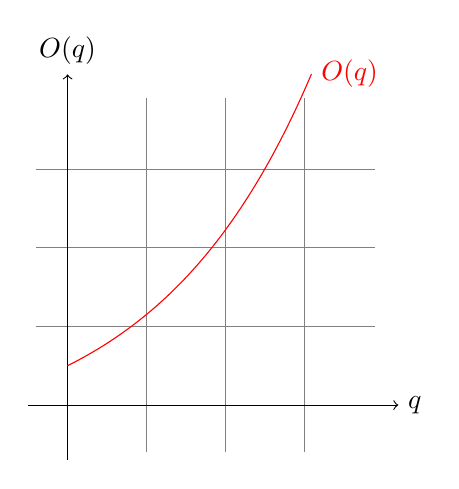
\begin{tikzpicture}[domain=0:3.5]
         \draw[very thin,color=gray] (-0.4,-0.6) grid (3.9,3.9);
         \draw[->] (-0.5,0) -- (4.2,0) node[right] {$q$};
         \draw[->] (0,-0.7) -- (0,4.2) node[above] {$O(q)$};
         \draw[color=red] [domain=0:3.1,samples=200] plot(\x, {-0.5 + exp(\x/2)}) node[right] {$O(q)$};
     \end{tikzpicture}
\end{center}

Supposons que l'offre augmente suite à l'apparition de nouvelles technologies
qui réduisent les coûts de production. \\

Quelle affirmation parmi celles ci-dessous est correcte? \\

\begin{choices}
     \choice La courbe se déplace vers la gauche.
     \choice L'équilibre se déplace vers la droite sur la courbe, qui reste
     identique.
     \choice \label{right2} La courbe se déplace vers la droite.
     \choice L'équilibre se déplace vers la gauche sur la courbe, qui reste
     identique.
\end{choices}

\begin{solution}
     Les nouvelles technologies vont faire augmenter la quantité vendue, et cela
     à un prix moindre. La réponse correcte est donc la réponse
     \fbox{\ref{right2}}.
\end{solution}

\section{Question 3}

Dans un contexte sans risque, on considère un marché avec un taux d’intérêt de
\SI{10}{\percent} et on vous propose les 4 projets générant les flux de
trésorerie suivants (où un nombre négatif correspond à une dépense, et un
nombre positif à une entrée).

\begin{equation*}
     \begin{array}{|| c || c | c | c ||}
          \hline
              & t = 0 & t = 1 & t = 2 \\
          \hline
          \hline
          P_1 & -99   & 110   & 121   \\
          \hline
          P_2 & -100  & 110   & 122   \\
          \hline
          P_3 & -100  & 110   & 121   \\
          \hline
          P_4 & 0     & 0     & 122   \\
          \hline
     \end{array}
\end{equation*}

Classez-les du moins avantageux au plus avantageux : \\

\begin{choices}
     \choice $P_4 < P_3 < P_1 < P_2$.
     \choice $P_4 < P_3 < P_1 = P_2$.
     \choice $P_1 = P_2 < P_3 < P_4$.
     \choice \label{right3} $P_3 < P_2 = P_4 < P_1$.
\end{choices}

\begin{solution}
     Calculons pour chaque projet le bénéfice attendu. On trouve alors

     \begin{equation*}
     \setlength\arraycolsep{1.5pt}
       \begin{array}{l c r c r c r c l}
          P_1 & = & -99 & + & \frac{110}{1.1} & + & \frac{121}{1.21} & = & 101
          \phantom{.}\\
          P_2 & = & -100 & + & \frac{110}{1.1} & + & \frac{122}{1.21} & \approx
          & \num{100.826}\phantom{.}\\
          P_3 & = & -100 & + & \frac{110}{1.1} & + & \frac{121}{1.21} & = & 100
          \phantom{.}\\
          P_4 & = & 0 & + & 0 & + & \frac{121}{1.21} & \approx &
          \num{100.826}.
       \end{array}
     \end{equation*}

     On voit immédiatement que la réponse correcte est la réponse
     \fbox{\ref{right3}}.
\end{solution}

\section{Question 4}

L'installation et la mise en fonctionnement d'une usine de taille $\lambda$
coûte

\begin{align*}
     C_{\textnormal{F,}\lambda} = 2 + \lambda^2.
\end{align*}

À ce montant viennent s'ajouter des coûts de production : une usine de taille
$\lambda$ permet de produire une quantité $q$ pour un montant de

\begin{align*}
     C_{\textnormal{V,}\lambda} = q + \frac{q^3}{4\lambda}.
\end{align*}

Quel est le coût \textbf{moyen}, à long terme, pour la production de 10 unités?
\\


\begin{choices}
     \choice $6$.
     \choice $5$.
     \choice $16$.
     \choice \label{right4} $8.7$.
\end{choices}

\begin{solution}
     On additionne le coût variable et le coût fixe pour obtenir le coût total

     \begin{align*}
          C(q, \lambda) &= C_{\textnormal{V,}\lambda} +
          C_{\textnormal{F,}\lambda} \\
          &= q + \frac{q^3}{4 \lambda} + 2 + \lambda^2.
     \end{align*}

     Pour trouver la taille optimale de l'usine, on égale la dérivée par rapport
     à $\lambda$ à 0.

     \begin{align*}
          \pdv{C(q, \lambda)}{\lambda} &= -\frac{q^3}{4 \lambda^2} + 2 \lambda
          \\
          &= 0.
     \end{align*}

     On trouve donc

     \begin{align*}
          8 \lambda^3 &= q^3 \\
          \lambda &= 5.
     \end{align*}

     On peut maintenant remplacer $\lambda$ dans la fonction de coût total, et
     diviser par $q$ pour obtenir le coût moyen.

     \begin{align*}
          \frac{C(q, \lambda)}{q} &= 1 + \frac{q^2}{4 \lambda} + \frac{2}{q} +
          \frac{\lambda^2}{q} \\
          &= 1 + \frac{100}{20} + \frac{2}{10} + \frac{25}{10} \\
          &= 8.7.
     \end{align*}

     La bonne réponse est donc la réponse \fbox{\ref{right4}}.
\end{solution}

\section{Question 5}

Voici ci-dessous des courbes de coût marginal (noté $\cmarg$) et de
coût moyen (noté $\cmoy$). Quel graphe ne peut PAS correspondre à
un vrai couple coût marginal-coût moyen?

\begin{figure}[H]
     \centering
     \begin{tikzpicture}[domain=0:4.1]
         \draw[->] (-0.5,0) -- (4.2,0) node[right] {$q$};
         \draw[->] (0,-0.5) -- (0,3.5) node[above] {$\frac{C(q)}{q}$};
         \draw[color=red] [domain=0:4.1,samples=200] plot(\x, {0.5 + \x/4}) node[right] {$\cmoy$};
         \draw[color=blue] [domain=0:4.1,samples=200] plot(\x, {0.8 + \x/2}) node[right] {$\cmarg$};
     \end{tikzpicture}
     \caption*{Graphe 1.}
\end{figure}

\begin{figure}[H]
     \centering
     \begin{tikzpicture}[domain=0:4.1]
         \draw[->] (-0.5,0) -- (4.2,0) node[right] {$q$};
         \draw[->] (0,-0.5) -- (0,3.5) node[above] {$\frac{C(q)}{q}$};
         \draw[color=red] [domain=0:4.1,samples=200] plot(\x, {2 - ((\x-2.3)^2)/5}) node[right] {$\cmoy$};
         \draw[color=blue] [domain=0:2.3,samples=200] plot(\x, {2 - ((\x-2.3)^2)/7});
         \draw[color=blue] [domain=2.3:4.1,samples=200] plot(\x, {02 - ((\x-2.3)^2)/3}) node[right] {$\cmarg$};
     \end{tikzpicture}
     \caption*{Graphe 2.}
\end{figure}

\begin{figure}[H]
     \centering
     \begin{tikzpicture}[domain=0:4.1]
         \draw[->] (-0.5,0) -- (4.2,0) node[right] {$q$};
         \draw[->] (0,-0.5) -- (0,3.5) node[above] {$\frac{C(q)}{q}$};
         \draw[color=red] [domain=0:4.1,samples=200] plot(\x, {2 - ((\x-2.3)^2)/4}) node[right] {$\cmoy$};
         \draw[color=blue] [domain=0:4.1,samples=200] plot(\x, {2 - ((\x-2.3)^2)/8}) node[right] {$\cmarg$};
     \end{tikzpicture}
     \caption*{Graphe 3.}
\end{figure}

\begin{choices}
     \choice Le graphe 1.
     \choice Le graphe 2.
     \choice \label{right5} Le graphe 3.
     \choice Aucun des graphes.
\end{choices}

\begin{solution}
     En regardant la partie du troisième graphe où les coûts descendent, on voit
     que malgré le fait que le coût marginal $\cmarg$ soit plus grand que le
     coût moyen $\cmoy$, ce dernier descend quand même. C'est évidemment
     impossible, et la réponse correcte est donc \fbox{\ref{right5}}.
\end{solution}

\section{Question 6}

Sur un marché en monopole non discriminant, une firme en monopole fixe son
niveau de production à $\qopt$ afin de maximiser son profit. Le prix s’établit
alors à $\popt$. Cet état de l’économie est-il Pareto-optimal? \\

\begin{choices}
     \choice Oui, car il est suffisant de vérifier que cet équilibre maximise
     le surplus collectif, ce qui est le cas ici.
     \choice Non, car cet équilibre est moins avantageux pour les consommateurs
     qu’une situation où le monopole serait \textit{price-taker}.
     \choice Oui, car tout autre niveau de production ou de prix résulterait en
     une baisse du profit de l’entreprise.
     \choice \label{right6} Non, car la situation serait améliorée si le
     monopole vendait en plus de $\qopt$ une quantité additionelle à un prix
     inférieur à $\popt$.
\end{choices}

\begin{solution}
     Comme le monopole est non discriminant, on est certain de ne pas être dans
     une situation Pareto-optimale.

     En faisant l'hypothèse qu'il n'y a pas de coûts fixes (si il y en a le
     raisonnement est toujours valable mais les formules se compliquent), on a
     que le surplus du poducteur est égal au profit de celui-ci. Faisons
     également l'hypothèse que $\abs{\elasticity} > 1$.

     On sait également qu'en concurrence parfaite, le prix est égal au coût
     marginal. En monopole, le prix se trouve ainsi :

     \begin{equation*}
          \fdif{R}{q} = R_{\textnormal{m}} = p + q \fdif{p}{q},
     \end{equation*}

     où $R$ est la recette et $R_{\textnormal{m}}$ est la recette marginale.

     On sait que l'élasticité est donnée par

     \begin{equation*}
          \elasticity = \frac{\frac{\dif q}{q}}{\frac{\dif p}{p}}.
     \end{equation*}

     On a donc que

     \begin{align*}
          R_{\textnormal{m}} &= p + q \left(\frac{p}{q} \frac{1}{\elasticity}\right) \\
          &= p \left(1 + \frac{1}{\elasticity}\right).
     \end{align*}

     Comme à l'équilibre monopolistique, on a

     \begin{equation*}
          R_{\textnormal{m}} = \cmarg,
     \end{equation*}

     on a

     \begin{equation*}
          \cmarg = \pmon \left(1 + \frac{1}{\elasticity}\right)
     \end{equation*}

     ou encore

     \begin{equation*}
          \pmon = \frac{\cmarg}{1 + \frac{1}{\elasticity}}.
     \end{equation*}

     C'est bien en accord avec l'énoncé car $\elasticity < 0$, et le prix en
     monopole est donc supérieur au prix en concurrence parfaite.

     Le ratio entre le surplus du consommateur en monopole et en concurrence
     parfaite est donné par

     \begin{equation*}
          r = \frac{\surpluscons^{\mathsc{mon}}}{\surpluscons^{\mathsc{cp}}} =
          \left(\frac{1}{1+\frac{1}{\elasticity}}\right)^{\elasticity+1}.
     \end{equation*}

     Le profit en monopole est donné par

     \begin{equation*}
          \pi^{\mathsc{mon}} =
          \left(\frac{\elasticity}{\elasticity+1}\right)^{\elasticity}
          \surpluscons^{\mathsc{cp}}.
     \end{equation*}

     En concurrence parfaite, le profit est nul (ce qui ne veut pas dire que
     les producteurs n'ont pas de revenu).

     Le surplus social (producteurs + consommateurs) en concurrence parfaite
     est donc égal au surplus du consommateur. En monopole, cependant, on perd
     une partie du surplus du consommateur, mais on gagne au niveau du profit.

     \begin{equation*}
          \surplus^{\mathsc{mon}} = \left( \left(\frac{1}{1+\frac{1}{\elasticity}}\right)^{\elasticity+1} + \left(\frac{\elasticity}{\elasticity+1}\right)^{\elasticity}
          \right) \surplus^{\mathsc{cp}}.
     \end{equation*}

     Pour $\elasticity < -1$, cela implique que le surplus social en monopole
     est inférieur à celui en concurrence parfaite. Si on vend plus à un prix
     moindre, on augmentera le surplus social. La bonne réponse est donc la
     réponse \fbox{\ref{right6}}.
\end{solution}

\section{Question 7}

On considère un marché des chaussures de sport : plusieurs firmes sont
présentes, et chacune projette une image légèrement différente des autres, et
plait donc plus à certains consommateurs qu’à d’autres. Les consommateurs
favoriseront donc certaines marques, mais resteront néanmoins sensibles aux
différences de prix.\\

En conséquence, la demande pour une marque de chaussures dépend à la fois du
prix de cette marque et du prix des autres marques sur le marché. Il s’agit
donc d’une situation de concurrence monopolistique.\\

Les firmes peuvent librement entrer et sortir du marché, et on suppose que
toutes les firmes, présentes ou potentiellement présentes sur le marché, sont
similaires : elles ont la même fonction de coût total, et font face à une même
réaction de la demande par rapport à des variations de leur prix ou du prix des
autres.\\

On suppose que l’équilibre de long terme est atteint, et en particulier que
plus aucune firme ne souhaite entrer sur le marché ou le quitter. \\

Quelle affirmation parmi celles ci-dessous est correcte? \\

\begin{choices}
     \choice Le prix est approximativement égal au coût marginal pour chaque
     firme.
     \choice Le prix peut être significativement différent du coût moyen et du
     coût marginal, pour chaque firme.
     \choice \label{right7} Le prix est approximativement égal au coût moyen
     pour chaque firme.
     \choice Le prix est approximativement égal au coût moyen et au coût
     marginal pour chaque firme.
\end{choices}

\begin{solution}
     L'équilibre de long terme est atteint, et afin de ne pas avoir de pertes,
     il faut que le profit soit à peu près nul. Comme le profit est égal
     à la différence entre les recettes totales et les coûts totaux, il faut que

     \begin{alignat*}{2}
          &\pi_i &&\approx 0\\
          \iff& R_i - C_i &&\approx 0\\
          \iff& R_i &&\approx C_i\\
          \iff& p \qi &&\approx C_i\\
          \iff& p &&\approx \frac{C_i}{\qi}\\
          \iff& p &&\approx C_{\textnormal{M,}i}.
     \end{alignat*}

     Le prix est donc approximativement égal au coût moyen pour chaque firme
     (réponse \fbox{\ref{right7}}).
\end{solution}

\section{Question 8}

Quelle phrase est correcte parmi celles ci-dessous à propos de l’utilité et du
surplus en économie?\\

\begin{choices}
     \choice L’utilité est une fonction, généralement croissante, décrivant la
     quantité de bien pouvant être acquise par le consommateur pour une unité de
     prix (dollars, euros,\dots). Le surplus du consommateur indique alors la
     quantité de bien excédentaire obtenue en payant le prix du marché.

     \choice \label{right8} L’utilité est une fonction, généralement
     croissante, décrivant la valeur (monétaire) qu’une quantité de bien
     représente pour un consommateur. Le surplus du consommateur est la
     différence entre l’utilité totale qu’il retire d’une quantité de bien et
     le prix total qu’il paye pour l’obtenir.

     \choice L’utilité est une mesure générale de la productivité du
     travailleur au sein d’une entreprise et peut être calculée par le rapport
     entre la valeur des biens qu’il produit et le salaire qu’il reçoit. Le
     surplus du producteur désigne la différence entre l’ensemble de la valeur
     produite par les travailleurs et leur salaire total.

     \choice L’utilité est la partie des dépenses qu’un consommateur effectue
     pour acquérir des biens essentiels (survenant à des besoins essentiels),
     dont l’élasticité est typiquement faible. Le surplus est la partie des
     dépenses qu’un consommateur effectue en vue d’acquérir des biens
     non essentiels ou de luxe, dont l’élasticité est typiquement plus
     importante.
\end{choices}

\begin{solution}
     Il s'agit simplement des définitions de l'utilité et du surplus. La
     réponse \fbox{\ref{right8}} est la bonne.
\end{solution}

\section{Question 9}

Une firme a une fonction de coût

\begin{equation*}
     C(q) = 1 + q + \frac{q^2}{2} \textnormal{ pour } q > 0 \textnormal{ et }
     C(0) = 0.
\end{equation*}

Si la firme est \textit{price-taker}, quel est le prix sur le marché à partir
duquel la firme a intérêt à produire une quantité positive?\\

\begin{choices}
     \choice $\frac{5}{2}$.

     \choice $1$.

     \choice \label{right9} $1 + \sqrt{2}$.

     \choice $\sqrt{2}$.
\end{choices}

\begin{solution}
     La firme veut que son profit soit maximal. Si elle ne fait rien, elle n'a
     pas de coûts (ni de recettes évidemment). Il faut donc que son profit soit
     strictement positif pour qu'elle investisse.

     \begin{align*}
          C(q) &= 1 + q + \frac{q^2}{2}\\
          \iff \fdif{C(q)}{q} &= 1 + q.
     \end{align*}

     On a donc $p = 1 + q$, ou encore $O(q) = 1 + q$, si $O(q)$ est définie.

     La contrainte sur le profit devient

     \begin{alignat*}{2}
          &pq - C(q) &&> 0\\
          \iff &(1 + q)q - 1 - q - \frac{q^2}{2} &&> 0\\
          \iff &-1 + \frac{q^2}{2} &&> 0\\
          \iff &q &&> \sqrt{2}\\
          \iff &p &&> 1 + \sqrt{2}.
     \end{alignat*}

     Le prix minimal est donc $p = 1 + \sqrt{2}$, c'est-à-dire la réponse
     \fbox{\ref{right9}}.
\end{solution}

\section{Question 10}

Une entreprise en monopole sur un marché a une fonction de demande

\begin{align*}
     D_1(q_1) = 20 - q_1.
\end{align*}

Sa fonction de coût est

\begin{align*}
     C(q) = \frac{q^2}{3}.
\end{align*}

Elle souhaite étendre ses activités au pays voisin dans lequel ne se trouve pas
de concurrent et dont le marché est décrit par la fonction

\begin{align*}
     D_2(q_2) = 50 - \frac{1}{2} q_2.
\end{align*}

L’entreprise a l’intention de vendre son produit au même prix sur les deux
marchés et considère donc les deux pays comme un seul grand marché. Donnez une
expression de la courbe de demande $D(q)$ de ce grand marché \textit{pour des valeurs $q$ proches de} 45.\\

\begin{choices}
     \choice \label{right10} $50 - \frac{1}{2}q$.

     \choice $70 - \frac{3}{2}q$.

     \choice $40 - \frac{1}{3}q$.

     \choice La fonction courbe de demande n’est pas/plus définie pour des
     valeurs proches de 45.
\end{choices}

\begin{solution}
     En observant la fonction de demande du second marché, on remarque que le
     prix sur celui-ci est plus élevé que sur le premier marché tant que $q_2
     < 60$. Comme $q \approx 45$, on se trouve dans ce cas et la firme devrait
     donc vendre tout son produit sur le deuxième marché. La fonction de
     demande devient alors la fonction de demande de ce marché, c'est-à-dire
     $50 - \frac{1}{2}q$, ou encore la réponse \fbox{\ref{right10}}.
\end{solution}

\section{Question 11}

Une firme possède deux usines dont les fonctions de coût sont respectivement

\begin{align*}
     C_1(q_1) = q_1 + \ln(1 + q_1) \qquad \textnormal{et} \qquad C_2(q_2) =
     q_2 + \ln(1 + q_2).
\end{align*}

(où $\ln$ est le logarithme népérien). La firme souhaite produire $q$ unités et
répartir la production de façon optimale entre les deux usines. Que vaudra le
coût total?\\

\begin{choices}
     \choice Le coût total sera inférieur à $q$.

     \choice $q + 2 \ln(1+\frac{q}{2})$.

     \choice \label{right11} $q + \ln(1 + q)$.

     \choice Le coût total sera supérieur à $2q$.
\end{choices}

\begin{solution}
     Les coûts marginaux sont les suivants :

     \begin{align*}
          C_{\textnormal{m,}1}(q_1) &= 1 + \frac{1}{1+q_1}\\
          C_{\textnormal{m,}2}(q_2) &= 1 + \frac{1}{1+q_2}.
     \end{align*}

     On remarque que plus $q_i$ est grand, mieux c'est, car le coût marginal
     diminue (graphiquement, la courbe s'applatit plus on avance vers les
     abscisses élevées). On a donc intérêt à produire toutes les $q$ unités dans
     la même usine. Le coût total est alors égal au coût d'une seule usine, ou
     bien $C(q) = q + \ln(1 + q)$, la réponse \fbox{\ref{right11}}.
\end{solution}

\section{Question 12}

Suite à la levée d’une législation, un marché initialement réservé à un
monopole est rendu accessible à d’autres producteurs. On fait l’hypothèse que
ces producteurs ne s’allient pas contre le monopole, ils n’acquièrent donc pas
suffisamment de pouvoir pour influencer le prix et se comportent chacun en
price-taker. \\

Le monopole est parvenu à estimer la fonction d’offre globale de ses
concurrents (établissant donc le lien entre la quantité totale mise sur le
marché par ses concurrents et le prix sur le marché) :

\begin{align*}
     O_{\textnormal{c}}(q) = 40 + 6q.
\end{align*}

Il connaît également la fonction de demande du marché.

\begin{align*}
     D(q) = 100 - 3q,
\end{align*}

ainsi que sa propre fonction de coût

\begin{align*}
     C_{\mathsc{t}}^{\mathsc{mon}}(q) = 30 + 60q + \frac{q^2}{2}.
\end{align*}

Quelle quantité doit-il mettre sur le marché pour optimiser son profit à
l'équilibre? \\

\begin{choices}
     \choice \label{right12} $4$.

     \choice $5$.

     \choice $\frac{40}{7}$.

     \choice $\frac{20}{3}$.
\end{choices}

\begin{solution}
     Les concurrents sont \textit{price-takers}. On sait donc que l'offre est
     égale à la demande.

     On trouve donc

     \begin{align*}
          40 + 6q_{\textnormal{c}} &= 100 - 3q_{\textnormal{c}} -
          3q^{\mathsc{mon}}\\
          q_{\textnormal{c}} &= \frac{20 - q_{\textnormal{c}}}{3}.
     \end{align*}

     Le monopole connaît cette valeur, et va l'utiliser pour optimiser son
     profit :

     \begin{align*}
          \pi^{\mathsc{mon}}(q^{\mathsc{mon}}) &= (100 - 3q_{\textnormal{c}} - q^{\mathsc{mon}})
          q^{\mathsc{mon}} - 30 - 60 q^{\mathsc{mon}} -
          \frac{(q^{\mathsc{mon}})^2}{2}\\
          &= (100 - 20 + q^{\mathsc{mon}} - 3 q^{\mathsc{mon}}) - 30 - 60
          q^{\mathsc{mon}} - \frac{(q^{\mathsc{mon}})^2}{2}.
     \end{align*}

     On maximise ce profit et on trouve donc que

     \begin{align*}
          \fdif{\pi^{\mathsc{mon}}(q^{\mathsc{mon}})}{q^{\mathsc{mon}}} = 80 - 4 q^{\mathsc{mon}} - 60 - q^{\mathsc{mon}} = 0.
     \end{align*}

     En résolvant cette équation, on trouve que $q^{\mathsc{mon}} = 4$,
     c'est-à-dire la réponse \fbox{\ref{right12}}.
\end{solution}

\section{Question 13}

Sur un marché en monopole, les fonctions de demande et de coût sont données par

\begin{align*}
     D(q) = 40 - 2q, \qquad \qquad C(q) = 40 + 2q.
\end{align*}

Le monopole choisit librement le prix et/ou la quantité qu’il met sur le
marché, mais une taxe est imposée en raison de ce monopole. Parmi les quatre
situations suivantes, laquelle mènera au plus grand surplus pour les
consommateurs?\\

(Note : le produit de la taxe est employé pour le bien commun, mais ne fait pas
partie ici du surplus des consommateurs.)\\

\begin{choices}
     \choice Le consommateur doit payer une taxe fixe de 2 euros par unité
     achetée.

     \choice \label{right13} L'État taxe \SI{50}{\percent} du profit de la
     firme.

     \choice La firme doit payer une taxe fixe de 2 euros par unité vendue.

     \choice L’État taxe la moitié de la recette (pour chaque euro payé par un
     consommateur, l’état prend 50 cents).
\end{choices}

\begin{solution}
     On voit immédiatement qu'il n'est pas nécessaire de calculer les valeurs
     pour le premier et le troisième cas, car comme le producteur peut choisir
     la quantité, taxer le producteur ou le consommateur revient exactement au
     même. Si ils ont le même surplus, et qu'il n'y a qu'une seule bonne
     réponse, aucun des deux ne peut être juste. À titre d'exercice, voici
     néanmoins la résolution :

     \begin{align*}
          \pi(q) &= (40 - 2q)q - 40 - 2q - 2q\\
          \iff \fdif{\pi(q)}{q} &= 36 - 4q\\
          &= 0.
     \end{align*}

     On trouve donc $\qopt_{1,3} = 9$, qu'on remplace dans la formule du surplus
     du consommateur pour trouver

     \begin{align*}
          S_{\textnormal{c,}1,3} &= \int_0^{9} (40 - 2\tilde{q}) \dif \tilde{q}
          - (40 - 2 \cdot 9) 9\\
          &= 81.
     \end{align*}

     Dans le second cas, on trouve le profit suivant :
     \begin{align*}
          \pi(q) &= \frac{1}{2} \left((40 - 2q)q - 40 - 2q\right)\\
          \iff \fdif{\pi(q)}{q} &= 20 - 2q - 1\\
          &= 0.
     \end{align*}

     On résout cette dernière équation et on trouve que la quantité optimale est
     $\qopt_2 = \frac{19}{2}$. Le surplus du consommateur est alors

     \begin{align*}
          S_{\textnormal{c,}2} &= \int_0^{\frac{19}{2}} (40 - 2\tilde{q}) \dif \tilde{q}
          - \left(40 - 2 \cdot \frac{19}{2}\right) \frac{19}{2}\\
          &= 90.25.
     \end{align*}

     Pour le quatrième cas, on sait que la recette totale est donnée par

     \begin{align*}
          R(q) &= \frac{1}{2}(40 - 2q^2).
     \end{align*}

     On calcule alors

     \begin{align*}
          \cmarg &= \tilde{R_{\textnormal{m}}}\\
          \iff 2 &= 20 - 2q.
     \end{align*}

     On trouve $\qopt_4 = 9$ et

     \begin{align*}
          S_{\textnormal{c,}4} &= \int_0^{9} (40 - 2\tilde{q}) \dif \tilde{q}
          - (40 - 2 \cdot 9) 9\\
          &= 81.
     \end{align*}

     On voit bien que le deuxième choix est optimal et la bonne réponse est donc
     la réponse \fbox{\ref{right13}}.
\end{solution}

\section{Question 14}

Une firme en monopole vend une quantité $\qopt$ d’un bien, à un prix qui
s’établit à $\popt$. On suppose que la fonction de demande est suffisament
régulière, et on constate que l’élasticité au prix du bien est de $-1$ autour
du prix $\popt$.\\

Quelle affirmation parmi les suivantes est correcte?\\

\begin{choices}
     \choice \label{right14} Une faible variation de la quantité $\qopt$ mise
     sur le marché n’aura pratiquement aucun impact sur les recettes.
     (\textit{C’est-à-dire : la dérivée des recettes par rapport à la quantité
     produite est nulle.})

     \choice Une faible diminution de la quantité $\qopt$ mise sur le marché
     mènera à un prix moins élevé. (\textit{C’est-à-dire : la dérivée du prix
     par rapport à la quantité produite est positive.})

     \choice  Une faible augmentation de la quantité mise sur le marché mènera
     à un prix moins élevé mais à des recettes plus élevées.
     (\textit{C’est-à-dire : la dérivée du prix par rapport à la quantité
     produite est négative, mais la dérivée des recettes par rapport à la
     quantité produite est positive.})

     \choice La firme a intérêt à légèrement augmenter sa production $\qopt$.
     (\textit{C’est-à-dire : la dérivée du profit par rapport à la quantité
     produite est positive.})
\end{choices}

\begin{solution}
     Dérivons les recettes par rapport à la quantité.

     \begin{align*}
          \fdif{R(p,q)}{q} &= \fdif{(pq)}{q}\\
          &= \fdif{p}{q}q + p\\
          &= \frac{p}{\elasticity} + p\\
          &= -p + p\\
          &= 0.
     \end{align*}

     La dérivée des recettes par rapport à la quantité produite est nulle, et la
     bonne réponse est donc la réponse \fbox{\ref{right14}}.
\end{solution}

\section{Question 15}

Une firme achète une machine à \num{5000} euros à l’année 0. Suite à un accord
avec le fournisseur, elle ne devra en payer le prix qu’à l’année 1.\\

Parmi les affirmations ci-dessous à propos de l’effet comptable de cette
opération, laquelle est correcte?\\

\begin{choices}
     \choice \label{right15} Cette opération a pour effet d’augmenter à l’année
     0 la valeur du passif et la valeur de l’actif de \num{5000} euros.

     \choice Cette opération a pour effet à l’année 1 de transférer \num{5000}
     euros du passif vers l’actif.

     \choice Cette opération a pour effet à l’année 0 de transférer \num{5000}
     euros du passif vers l’actif.

     \choice Cette opération n’a pas d’impact à l’année 0 sur la valeur totale
     de l’actif ni sur la valeur totale du passif.
\end{choices}

\begin{solution}
     Le tableau de bilan donnant l'état de l'entreprise à l'année 0 se
     construit ainsi :

     \begin{center}
          \begin{tabular}{c || c}
               Actif & Passif \\
               Ensemble des biens/droits de l'entreprise. & Ressources
               de l'entreprise. \\
               \hline
               \hline
               Machine (\num{5000} euros) & Dette (\num{5000} euros)
          \end{tabular}
     \end{center}

     La valeur du passif et la valeur de l'actif sont donc augmentées de
     \num{5000} à l'année 0; c'est-à-dire la réponse \fbox{\ref{right15}}.
\end{solution}

\section{Question 16}

Un ami est venu vous demander de lui prêter de l’argent pour l’aider à lancer
sa startup. Il prétend être sûr de pouvoir vous rembourser la somme complète
dans un an. Cependant, vous le connaissez depuis longtemps et vous avez peu
confiance en la réussite de son projet. Vous estimez que sa startup a une
probabilité ($\frac{1}{5}$) de faire faillite endéans l’année et vous savez que
dans ce cas il ne sera pas en mesure de vous rembourser le moindre sou. Vous
acceptez finalement de lui prêter la somme de 400 euros aux conditions
suivantes :

\begin{itemize}
     \item si dans un an la startup n’a pas encore fait faillite, il vous
     remboursera à cette date 540 euros;

     \item par contre, si la startup fait faillite d’ici-là, il ne vous
     remboursera rien.
\end{itemize}

Sachant que vous agissez de manière neutre par rapport au risque, quel est le
taux sans risque du marché?\\

\begin{choices}
     \choice $\SI{35}{\percent}$.

     \choice Cette situation ne correspond à aucun taux d'intérêt strictement
     positif.

     \choice $\SI{12}{\percent}$.

     \choice \label{right16} $\SI{8}{\percent}$.
\end{choices}

\begin{solution}
     Il faut que

     \begin{align*}
          -400(1 + x) + 540 \frac{4}{5} &= 0\\
          x &= 0.08.
     \end{align*}

     Le taux sans risque est donc de $\SI{8}{\percent}$, ou bien la réponse
     \fbox{\ref{right16}}.
\end{solution}

\section{Question 17}

Dans un marché caractérisé par une fonction de demande

\begin{align*}
     D(q) = 48 - q,
\end{align*}

deux firmes sont en situation d’oligopole. La firme A apprend que sa
concurrente, la firme B, projette de systématiquement produire le double de ses
futures productions (le double de A). Sachant que la firme A a des coûts de
production décrits par la fonction suivante :

\begin{align*}
     C_1 = q_1^2,
\end{align*}

qu’elle ignore la fonction de coût de la firme B, mais que celle-ci est
strictement inférieure à celle de A, quel est le profit maximal que la firme A
peut espérer dégager dans cette situation?\\

\begin{choices}
     \choice $\left(\frac{48}{5}\right)^2$.

     \choice $128$.

     \choice \label{right17} $144$.

     \choice $0$, elle ne peut pas dégager un bénéfice dans
     cette situation.
\end{choices}

\begin{solution}
     La fonction de demande totale est donnée par :

     \begin{align*}
          D(q) = 48 - q_1 - q_2.
     \end{align*}

     On sait que $q_2 = 2 q_1$. Le profit est donné par

     \begin{align*}
          \pi(q_1) = q_1 (48 - 3 q_1) - q_1^2.
     \end{align*}

     On dérive cette expression par rapport à $q_1$ pour trouver la quantité
     optimale.

     \begin{align*}
          \fdif{\pi(q_1)}{q_1} &= 48 - 6 q_1 - 2q_1\\
          &= 0\\
          \iff q_1 &= 6.
     \end{align*}

     En remplaçant cette valeur dans la formule du profit, on obtient

     \begin{align*}
          \pi(q_1) &= 6 (48 - 3 \cdot 6) - 6^2\\
          &= 144.
     \end{align*}

     La bonne réponse est donc la réponse \fbox{\ref{right17}}.
\end{solution}

\section{Question 18}

Un marché sur lequel la fonction de demande est

\begin{align*}
     D(q) = 10 - q
\end{align*}

est en situation de duopole. Les deux producteurs se comportent en followers.
Leurs fonctions de coût sont données par

\begin{align*}
     C_1(q_1) = 8 q_1 \qquad \textnormal{et} \qquad C_2(q_2) = 10 + 5 q_2.
\end{align*}

Que vaut la quantité totale échangée à l’équilibre?\\

\begin{choices}
     \choice $\frac{11}{4}$.

     \choice \label{right18} $\frac{5}{2}$.

     \choice $\frac{7}{3}$.

     \choice $\frac{8}{3}$.
\end{choices}

\begin{solution}
     Les deux fonctions de profit sont données par

     \begin{align*}
          \pi_1(q_1,q_2) &= (10 - q_1 - q_2) q_1 - 8 q_1\\
          \pi_2(q_1,q_2) &= (10 - q_1 - q_2) q_2 - 10 - 5q_2.
     \end{align*}

     On veut annuler les dérivées de ces fonctions car les firmes maximisent
     leur profit.

     \begin{align*}
          \pdv{\pi_1(q_1,q_2)}{q_1} &= 10 - 2q_1 - q_2 - 8 = 0\\
          \pdv{\pi_2(q_1,q_2)}{q_2} &= 10 - q_1 - 2q_2 - 5 = 0.
     \end{align*}

     On simplifie ces équations pour obtenir le système suivant

     \begin{align*}
          2q_1 + q_2 = 2\\
          q_1 + 2q_2 = 5.
     \end{align*}

     La solution du système est le point $(q_1, q_2) =
     (-\frac{1}{3},\frac{8}{3})$. Comme $q_1$ est négatif, on le met égal à zéro
     et on résout de nouveau, uniquement pour $q_2$.

     \begin{align*}
          \pi_2(q_2) &= (10 - q_2) q_2 - 10 - 5q_2.
     \end{align*}

     Encore une fois, la dérivée par rapport à la quantité doit être nulle. On
     trouve donc

     \begin{align*}
          \fdif{\pi_2(q_2)}{q_2} = 10 - 2q_2 - 5 = 0.
     \end{align*}

     On résout cette équation pour trouver $q_2 = \frac{5}{2}$.

     Comme $q = q_1 + q_2$, on a $q = \frac{5}{2}$ (réponse
     \fbox{\ref{right18}}).
\end{solution}

\section{Question 19}

Deux firmes 1 et 2 sont présentes sur un marché. Leurs fonctions de coût sont

\begin{align*}
     C_1(q_1, q_2) &= 5 + q_1 + q_1(q_1 + q_2),\\
     C_2(q_1, q_2) &= 5 + q_2 + q_2(q_1 + q_2),
\end{align*}

où $q_1$ est la quantité produite par la première firme et $q_2$ celle produite
par la seconde. La fonction de demande sur ce marché est

\begin{align*}
     D(q) = 22 - q.
\end{align*}

Que vaut le prix à l’équilibre si les firmes se comportent en price-takers?\\

\begin{choices}
     \choice $16.75$.

     \choice Aucune de ces réponses.

     \choice $16$.

     \choice \label{right19} $13.6$.
\end{choices}

\begin{solution}
     Les profits des deux firmes sont donnés par

     \begin{align*}
          \pi_1(q_1,q_2) &= D(q) q_1 - 5 - q_1 - q_1 (q_1 + q_2)\\
          \pi_2(q_1,q_2) &= D(q) q_2 - 5 - q_2 - q_2 (q_1 + q_2).
     \end{align*}

     On doit annuler leurs dérivées par rapport aux quantités pour maximiser.

     \begin{align*}
          \pdv{\pi_1(q_1,q_2)}{q_1} &= D(q) - 1 - 2q_1 - q_2 = 0\\
          \pdv{\pi_2(q_1,q_2)}{q_2} &= D(q) - 1 - q_1 - 2q_2 = 0.
     \end{align*}

     On trouve donc le système d'équations suivant :

     \begin{align*}
          D(q) &= 1 + 2q_1 + q_2\\
          D(q) &= 1 + q_1 + 2q_2.
     \end{align*}

     En remplaçant la fonction $D(q)$ par sa valeur, et comme on sait que les
     quantités produites par chaque firme seront égales car les firmes sont
     parfaitement identiques, on trouve alors

     \begin{align*}
          21 &= 5q_1\\
          q_1 &= q_2 = 4.2.
     \end{align*}

     On remplace cela dans $D(q) = 22 - q_1 - q_2$ pour trouver le prix, qui est
     de $13.6$. La réponse \fbox{\ref{right19}} est donc la bonne.
\end{solution}

\section{Question 20}

En plusieurs endroits du monde au cours des 20 dernières années, des entités de
régulation des monopoles ont cessé d’utiliser la méthode de régulation dite
``cost-plus''. Celle-ci sera ici résumée par cette équation :

\begin{align*}
     s = \frac{p(q) \cdot q(K,L) - wL}{K}
\end{align*}

dans laquelle $p$ est le prix en fonction de la quantité produite, $K$ le
capital investi, $L$ le nombre d’unités de travail et $w$ le taux de salaire
associé. Une régulation correspond ici à placer une borne supérieure sur $s$.

Parmi les affirmations ci-dessous à propos des désavantages de cette méthode,
et donc des raisons qui peuvent mener à son abandon, laquelle est \textit{correcte}?\\

\begin{choices}
     \choice \label{right20} Cette méthode encourage l’entreprise à
     surinvestir.

     \choice Cette méthode n’encourage pas l’entreprise à optimiser le
     rendement unités de travail/salaire.

     \choice Cette méthode ne permet pas d’assurer l’équilibre budgétaire de
     l’entreprise.

     \choice Cette méthode entraîne des surproductions.
\end{choices}

\begin{solution}
     En augmentant fortement $K$, on fait diminuer $s$, et on s'éloigne donc de
     la borne supérieure imposée. Cette méthode encourage donc l'entreprise à
     surinvestir, ou bien la réponse \fbox{\ref{right20}}.
\end{solution}

\end{document}
